
\section{Singing}

Participation in rhythmic events.

Goal: for robot to participate in patterned activity in real time with a human partner

- Coordinated motor activity

- Vocalization: e.g. singing, proto-dialog

- Coordinated gesturing, tapping, rhythmic movement

For example, if a human starts humming or tapping something rhythmic in time or pitch, we'd like the robot to rapidly join in


Why?

Participation in rhythmic activity is a means to an end, rather than a goal in itself

Overall goal is to make machine learning on the robot more autonomous

Knowing the overall structure of an activity gives a "skeleton" upon which the specific objects and actions (potentially initially unmodeled) within that activity could be analysed.

Also, participating in activity is better than just observing it, since there is an implicit signalling of "comprehension" level

Ideally would be integrated with other behaviors (cross-reference IST imitation work, affordance exploitation)


(see previous deliverable, d N.N)

Update: work has now been applied in practice, to pitch perception/production experiment

Next step: 

- Apply across multiple signals

- Different aspects of speech sounds

- Arm movements, gesturing

- Exploit knowledge of structure for learning of parts


\subsection{Summary}

(spectrograms just show a low frequency range, to make the pitch visible).

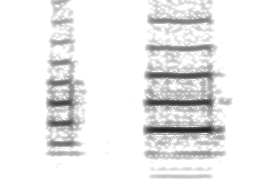
\includegraphics[height=2cm]{images/chico-output-separate-high-low}

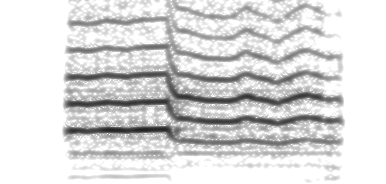
\includegraphics[height=2cm]{images/chico-output-pair-high-low}

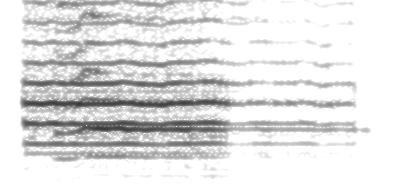
\includegraphics[height=2cm]{images/chico-output-ohm}

\subsection{Tone sequence}

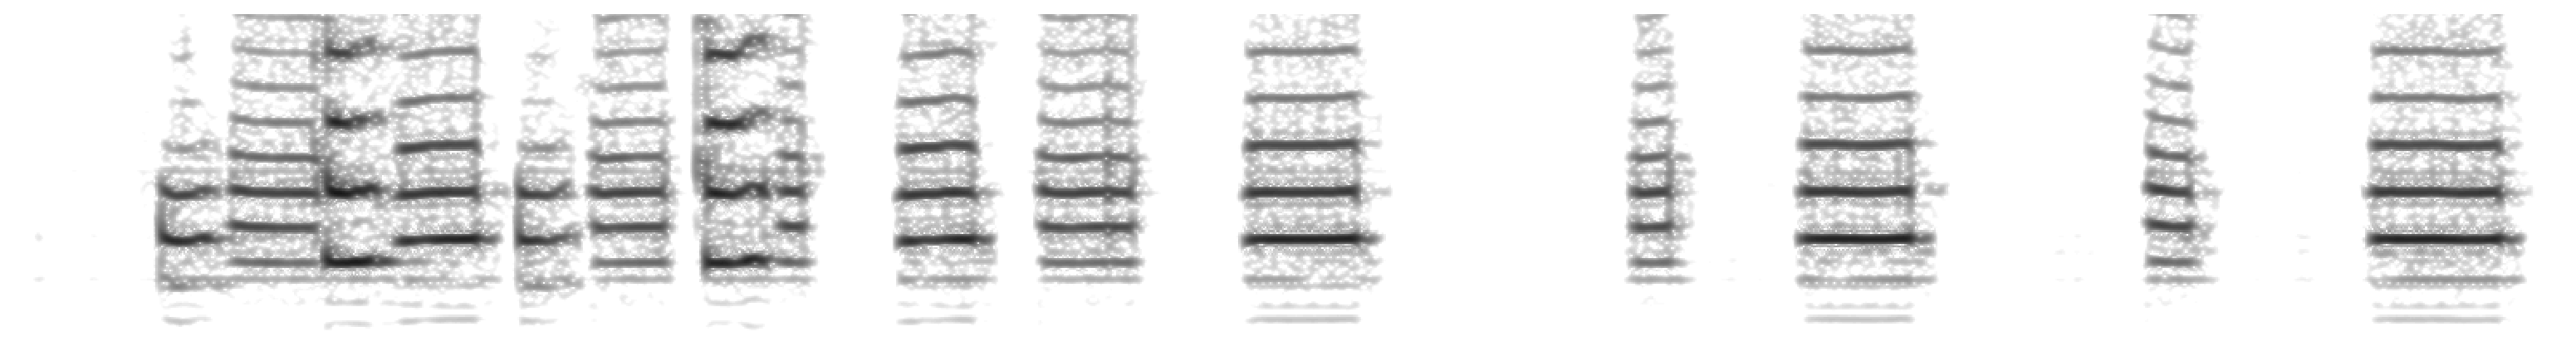
\includegraphics[height=2cm]{images/chico-separate-begin}

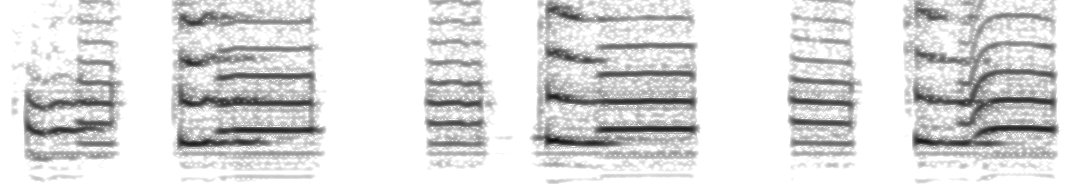
\includegraphics[height=2cm]{images/chico-separate-together}

\subsection{Prosodic unit}

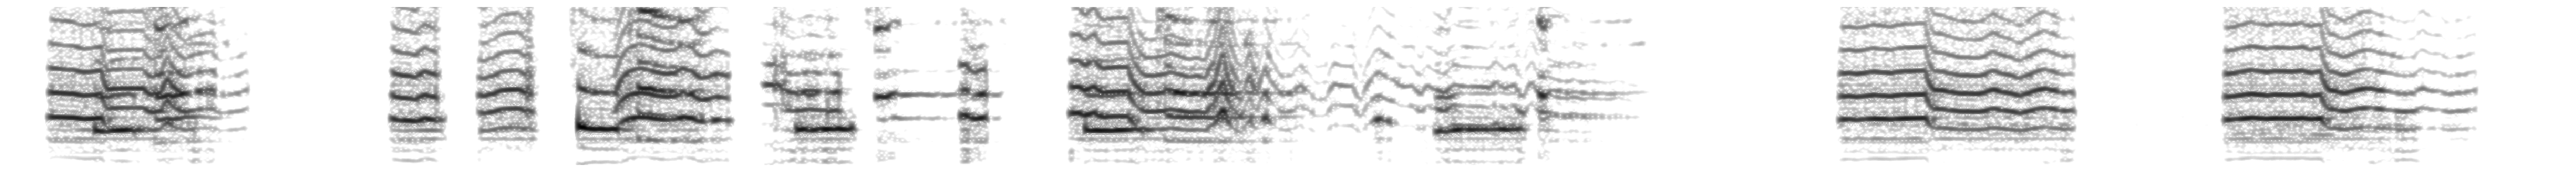
\includegraphics[height=1cm]{images/chico-pair}

\subsection{Ohm}

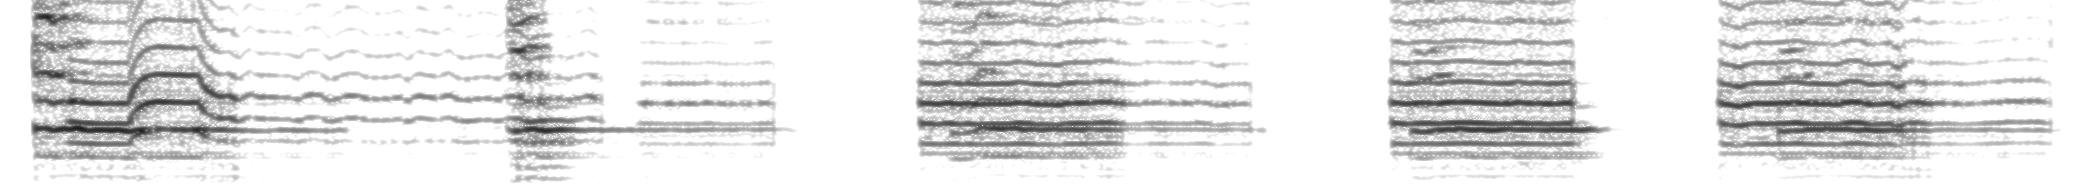
\includegraphics[height=1cm]{images/chico-ohm}




